\chapter{Design}
\label{sec:design}
In this chapter the design for the Camera Provisioning system will be laid out.
The goal of the system is to provide a solution which makes it possible to manage camera configurations.
The system allows the user to orchestrate parameters into different templates which can be assinged to a camera.
The design will contain both functional and technical specifications containing the descriptions of different components, requirements and supplemental diagrams and wireframes.
\section{Requirements}
In table \ref{tab:requirements} the requirements for the system have been defined. Requirements are tracked using an identifier starting with a letter followed by a
number and are listed in the ID column of table \ref{tab:requirements}. If the identifier starts with the letter 'B' or a 'U' they specify a business or user requirement respectively. If the identifier starts with a 'F' or 'NF' they specify a functional or non-functional system requirement respectively.
Requirements have been prioritized using the MoSCoW method \cite{noauthor_moscow_nodate}.
\begin{table*}[h]
    \centering
    \begin{tabulary}{\linewidth}{CLL}
        \textbf{ID} & \textbf{Requirement} & \textbf{MoSCoW}
    %%% Business requirements
        \\ \hline %% Check this with NF-7
        B1 & A camera can be configured by the user without detailed knowledge about the model being used & Must
        \\ \hline
        B2 & A camera configuration can be rolled back to any compatible version in history & Must
        \\ \hline
        B3 & The configuration changes must include auditing: show the author and timestamp & Must
        \\ \hline
        B4 & Translated parameters that are scaled to a particular value should be tuneable & Should
        \\ \hline
        B5 & The application has the option to show the user the differences between the config in the camera and the template & Must
    %%% User requirements
        \\ \hline
        U1 & A user can login using a username \& password & Could
        \\ \hline
        U2 & A user can change his credentials through the web interface & Could
        \\ \hline
        U3 & The template used for configuring cameras must include one setting representing a text-field and one setting representing a slider value & Should
        \\ \hline
        U4 & New settings can be added to the application without having to change the templates & Must
        \\ \hline
        U6 & The application must be able to handle one or more settings in a template that are not present in any of its parents & Should
        \\ \hline
        U7 & A user can interface with the system using a webbrowser & Should
        \\ \hline
        U8 & A user can create a new template with a specified parent template & Must
        \\ \hline
        U9 & A user shall be able to trigger the configuration on one or all cameras according to their template & Must
    %%% System requirements
        \\ \hline
        NF-1 & Communication with cameras are authenticated through HTTP Basic or Digest & Must
        \\ \hline
        NF-2 & The code must be compiled crossplatform & Must
        \\ \hline
        NF-3 & The codebase must be covered with linting. & Must
        \\ \hline
        NF-3 & The codebase shall be strongly typed. & Should
        \\ \hline
        NF-3 & All code shall be covered by unit tests & Must
        \\ \hline
        NF-4 & Templates and camera configuration are stored on disk in a human-readable/typeable format & Must
        \\ \hline
        NF-5 & Templates and camera configuration can be loaded from YAML files & Must
        \\ \hline %% TODO check this with Wouter. Not SMART
        NF-6 & The application should be exposed as a RestAPI and documented via OpenAPI & Should
        \\ \hline
        NF-7 & The templates must be camera independent. & Must
    \end{tabulary}
    \caption{Requirements}
    \label{tab:requirements}
\end{table*}

\section{General design}
At the conclusion of this project the prototype is handed over to the back-end team of BauWatch.
Since they will be further developing the prototype into a production ready system the choice was made to implement the system in Go as that programming language is their preferred language for new products fulfilling requirement NF-2.

\section{Templates}
The provisioning server will have a user interface through which a template can be configured.
A template in the context of this system is a collection of lists containing camera configuration options.
Templates can be built up from different layers where each layer can override parameters from the layer above.
This allows the user to define a template that is shared by a large amount of cameras but still provides more fine-tuned control for certain situations.
These cameras would still use all the settings from the parent template but would have a different setting for camera sensitivity.

\section{Datastructure}
Templates are represented in memory as a tree using dynamically allocated nodes that have pointers to one parent and zero or more children.
There is a single template that is considered to be the root node of the tree.
All templates that are added to the system will be a child of this root node.
The choice to represent the collection of templates as a tree is to solve the requirement of parameter inheritance.
Using this datastructure is an efficient method to enumerate the values of a template's parameters at configuration time.
A parameter can be found by traversing each parent node starting from the node representing the current template until a value for a given paramater is found.
The process of finding a paramater is depicted in figure TBD % TODO add figure
The best-case performance for a parameter lookup is O(1) in the case the parameter is already defined in the current template.
The worst-case performance of a lookup is O(n) where n is the number of templates to be traversed from the current node to the root node.
When a new template is instantiated, by creating a new one or loading one from YAML, that template has to be inserted at the correct place inside the tree.
The way this is achieved is to do a breadth-first search (BFS) in the tree where a match is identified using the name of the parent node.
Using BFS to find the parent node is more efficient than a depth-first search (DFS) as a template is more likely to inherit from a more generic template describing e.g. paramaters for a country than a more specific template representing paramaters for a specific building site. % TODO Proof?

\section{Multiple base templates} %TODO: Root template requires more intro?
While this design requires a single root template that all other templates inherit from, the design still allows the creation of multiple trees with independendant parameter sets.
This can be done by not setting any paramaters in the root template such that the templates directly below it don't have any parameters that can be inherited from the root template.
The children of the root template then become the first template to define the template effectively turning into root templates themselves while still being children of the actual root template.

\subsection{Parameters}
%TODO: How are the templates kept in memory. Describe the parameter interface
%TODO: How will stuff look in the main application
TBD Once I figure out how to properly abstract them in Go.
At the moment only integer parameters are supported.

Cameras can contain many different kinds of parameters. To handle these in a generic way some kind of abstraction needs to be done.
Parameters 

\section{Storing to file}
Templates are stored on disk as YAML formatted data. YAML was chosen because it is a plain text format that can be interpreted by humans while still being able to describe all attributes that make up a template. 
Due to the plain text nature this also allows the usage of tools like GNU diff to produce a view of the differences between two templates.
An example of a YAML-formatted template can be found in listing \ref{lst:template}.
The following data is used to describe a template in YAML:
\begin{itemize}
	\item name: The name of the template.
	\item parent: The name of the parent template this template should inherit from.
	\item parameters: A list of all the parameters contained in this template.
	\item type: A name that defines the type of a parameter.
	\item name: (under parameters): The name of the parameter.
	\item attributes: A generic list with data used to construct a paramater of the type in the `type` key.
\end{itemize}
\lstinputlisting[language=yaml,caption={Example template YAML},label={lst:template}]{format.yaml}

\section{Reading from file}
Templates are stored on disk with the name of the parent. When this file is reloaded to instantiate a template the system must be able to discover its
parent by its name. This can be achieved using a breadth-first search of the template tree.
The operation of loading a template and linking these to their parent is described in figure \ref{fig:inserttemplate}.

\begin{figure}[h!]
	\centering
	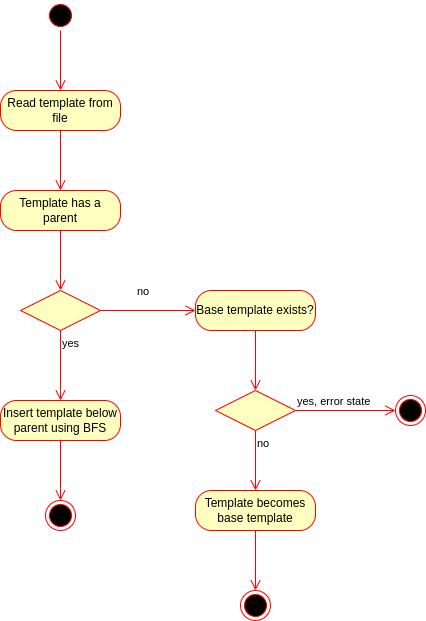
\includegraphics[scale=0.5]{insert_template_acty}
	\caption{Template insert operation}
	\label{fig:inserttemplate}
\end{figure}

\section{Keeping revision history}
In order to fullfill the ability to restore a template to a previous version a revision history is kept.
Templates are stored in a directory with the name of that template.
Inside that directory a template is stored as a file named with the revision number and the file extension (.yml).
This way the latest revision can be found by sorting the files by name in descending order.
When a template is reverted to a previous version the files will be sorted in the same manner and will be deleted until the revision to revert to is reached. An example of how this directory structure would be stored is seen in figure \ref{fig:diskstruct}

Storing templates in this manner has one flaw.
Namely that of sorting by name when more than 10 revisions have been made.
A solution to this problem could be to use leading zeroes to delay the problem or to sort on a different attribute, like file modification time.

One off the shelf solution for versioning files that cannot be ignored is git.
Git is originally intended to keep track of program source files but can also be used for other kinds of files.
The goals of git are speed, data integrity and distritbuted workflows.

Argument: Is git overkill? Why use it or the other suggested solution. Make a choice.

Design:
Each time a template is saved it is saved as a yaml file and committed in git.
A commit only modifies one file at a time.
A template can be reverted to an earlier commit.
Author information is entered at the login screen.
library available that implements porcelain functions.

\begin{figure}[h!]
	\centering
	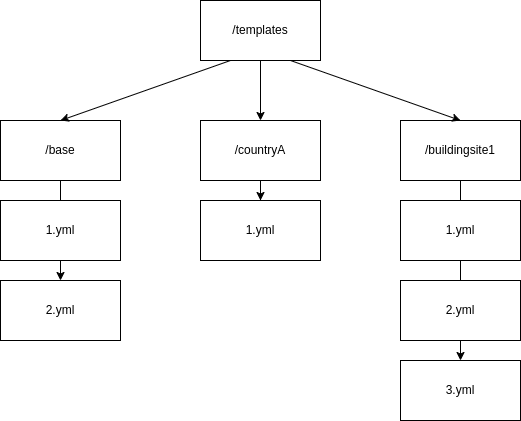
\includegraphics[scale=0.5]{yaml_dir_struct}
	\caption{Directory structure of templates and their revisions}
	\label{fig:diskstruct}
\end{figure}

\subsection{Camera interface}
The camera interface is a system component that sits between the template component and the cameras themselves. The purpose of this component
is to translate the settings from a template into an API call understood by the camera. Each camera can have a different API with potentially different interpretation of parameters. This component will map the parameter from the template to an appropriate value for that camera.
In order for a camera to accept new parameters they require a form of authentication. All cameras being used support both HTTP Basic and HTTP Digest authentication.
To successfully interface with the cameras one or both of these authentication methods must be supported by the camera interface component.

\subsection{Translating generic parameters to camera specific values}
As an example of translating a generic parameter to a camera specific value the detection sensitivity parameter is used.
For the Hikvision camera this is a value that can be configured between 0 and 100 in increments of 20.
For the VCA camera this works XXX. TBD: How does this work

Because these paramaters may behave differently between camera manufacturers and individual models the template paramater is divided into a couple of presets. The presets are labeled as low, medium, high and ultra. These predefined levels are used by the Camera API to map a parameter to a specific value for that camera. These values are implemented in such a way that extra levels can be introduced and their values adjusted to fine tune a cameras behavior.

\subsection{User interface}
The components of the system can be managed through a web interface.
They will allow the user to create a new template and add parameters to it as seen in figure \ref{fig:templatewireframe}.
The user should also be able to manage the relations between templates as well as registering new cameras to be managed by the system (TBD still).
\begin{figure}[h!]
	\centering
	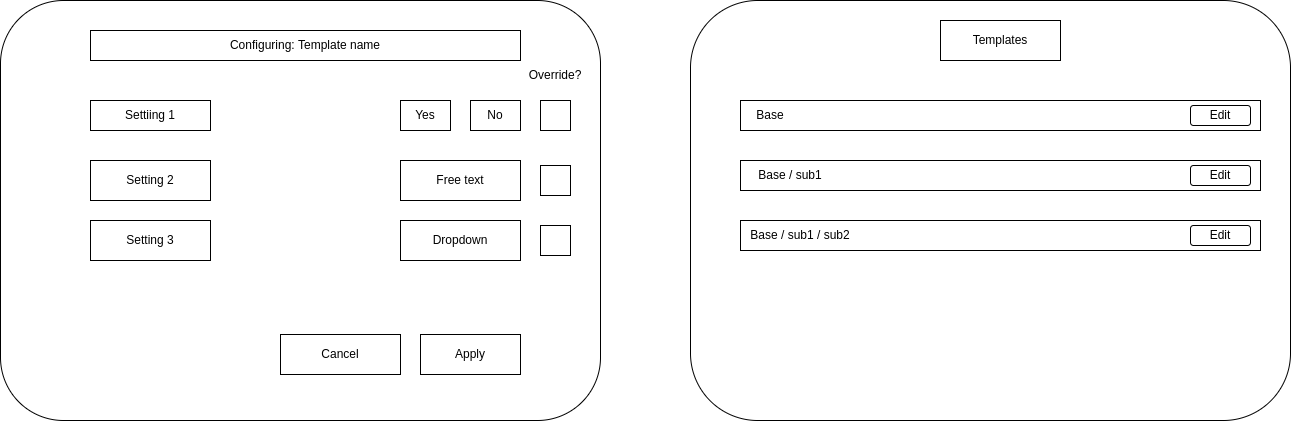
\includegraphics[scale=0.2]{wireframes}
	\caption{Template overview  wireframe}
	\label{fig:templatewireframe}
\end{figure}

\subsection{Design patterns}
TBD Integrate these where applicable instead of separately.

Design patterns are reusable solutions to commonly occurring software design problems. Design patterns are not ready made solutions that directly translate to machine readable code. Rather they are concepts that can be applied to solve a common problem in different situations. They may be seen as an intermediate between a programming paradigm (e.g. functional- or object-oriented programming) and
concrete algorithms. Design patterns can be divided in three categories, namely creational, behavioral and structural.

\subsubsection{Composite}
The composite pattern is a structural design pattern. With this design pattern objects can be grouped such that they are treated as a
single instance.

\subsubsection{Factory}
The factory method is a creational design pattern used for creating objects in a generic superclass that allows subclasses to change the
specific type of object that is created.
